\begin{center}
\bfseries{\large ТЕХНИЧЕСКИЙ ОТЧЁТ ПО ПРАКТИКЕ}
\end{center}

\section*{Архитектура}

Node JS - программная платформа, основанная на движке V8 (транслирующем JavaScript в машинный код), превращающая JavaScript из узкоспециализированного языка в язык общего назначения. Node.js добавляет возможность JavaScript взаимодействовать с устройствами ввода-вывода через свой API (написанный на C++), подключать другие внешние библиотеки, написанные на разных языках, обеспечивая вызовы к ним из JavaScript-кода.

Структура состоит из главного файла index.js, к которому посредством экспортирования модулей через require, написанных на языке JS, подключаются классы или функции, которые в дальшейнем можно использовать в приложении.

В основном стоит затронуть разделы text и search, в них прописаны маршруты, специальные функции middleware, которые имеют доступ к req и res, могут модифицировать их, передавать управление другим функциям. Зная требования, пользователь API может отправить по некому URL запрос, сервер найдет для него нужный обработчик, и через единичный или цепной middleware модифицирует запрос, сделает реквест в базу данных, сохранит данные или вернет требуемую информацию.

База данных mongodb выбрана не случайно, ее проще всего использовать в такой связке, так как она не является типичной листовой базой данных как mySQL, она не является принудительно реляционной, обладает динамикой изменения структур, поддержкой всех качеств JS, правильный перевод форматов, следовательно можно просто отдать базе данных структуру из JS, например Map(), и так же вернуть ее обратно, без какой либо модификации, что очень удобно.

При написании хотел использовать модуль http, но остановился на express, что он из себя представляет - фреймворк node js, максимально минималистичный, позволяет писать вышеупомянутые middleware обработчики. Главная проблема - он довольно медленный и не подходит для маленьких приложений.



\section*{Описание}

Описание маршрутов api.

post /text \{title:string data:string\} => \{\_id:string, title:string\} - публикация текста.

get /text/id => \{\_id:string, title:string, data:string\} - получение текста по id.

get /text => array of \{\_id:string, title:string, data:string\} - получения всей базы текста.

delete /text/id => string - удаление текста по id.

\vspace{10pt}

get /search/id \{pattern:string\} => \{result:number\} - проверка плагиата pattern по тексту id.

get /search \{title:string, pattern:string\} => \{result:number\} - проверка плагиата pattern по тексту title.

get /search \{titles:array of string, pattern:string\} => array of \{\_id:string, title:string, result:number\} - проверка плагиата pattern по текстам с title из titles.

get /search => array of \{\_id:string, title:string, result:number\} - проверка плагиата pattern по текстам из db.

\section*{Реализация}

Сервер написан на node js - платформа на движке v8, она дает нам возможность использовать фреймворки, такие как express и mongodb и все это на языке JS, что очень удобно, не приходится учить разные языки, для разных вещей.

express - фреймворк, дает возможность отслеживания запросов на сервер, простая нотация позволяет задать тип запроса, его переменные и данные, также система middleware помогает разбить участки кода на сегменты, что очень сильно облегчает дальнейшее чтение кода.

mongodb - дает нам два пути дальнейшего развития событий. Первый, создание локального хранилища, мы создаем файл .db, делаем привязку к нему через соединения клиента и теперь мы можем на старте сервера подгружать базу и использовать ее в наших целях.
Второй вариант, который выбрал я - учетная запись на mLab, где дается беспланое хранилище mongodb базы на 500 мб, что вполне хватит для разработки начальной идеи приложения. Чем это хорошо? Возможность сменить базу изменением одного файла конфига, меньшая нагрузка на локальную машину. База всегда поднята и готова к работе.
Также сервис предлагает отчетность по базе данных, просмотр ее содержимого, модификация и удаления данных, отчет о подключениях и скорости работы сети и правильность выполнения запросов. Имея локальную базу данных очень трудно залезть в базу и что то там поменять, при необходимости.

body-parser - библиотека для правильного отображения urlencoded формата, при передаче сообщения в таком формате.

nodemon (опционально) - linux утилита, позволяет избежать постоянного ручного поднятия и отключения сервера, утилита следит за изменениями файлов проекта, и как только файл изменил содержимое, автоматически компилирует код и поднимает сервер в рабочее состояние. Крайне полезный инструмент. Также позволяет отследить ошибки при написании, выдавая правильный и информативный отчет на стадии компиляции.

npm - менеджер пакетов node js, нужен для отладки конфигураций пакетов и версий node js, формирует настройки, позволяет расширять фреймворки, добавлять новые в проект, регулирует версии, сообщает об ошибках и несовместимостях.

\section*{Тестирование}

Тестирование и отладка проводится с помощью бесплатной программы Postman, имея адрес сервера позволяет отправлять запросы в разных форматах с любыми параметрами.

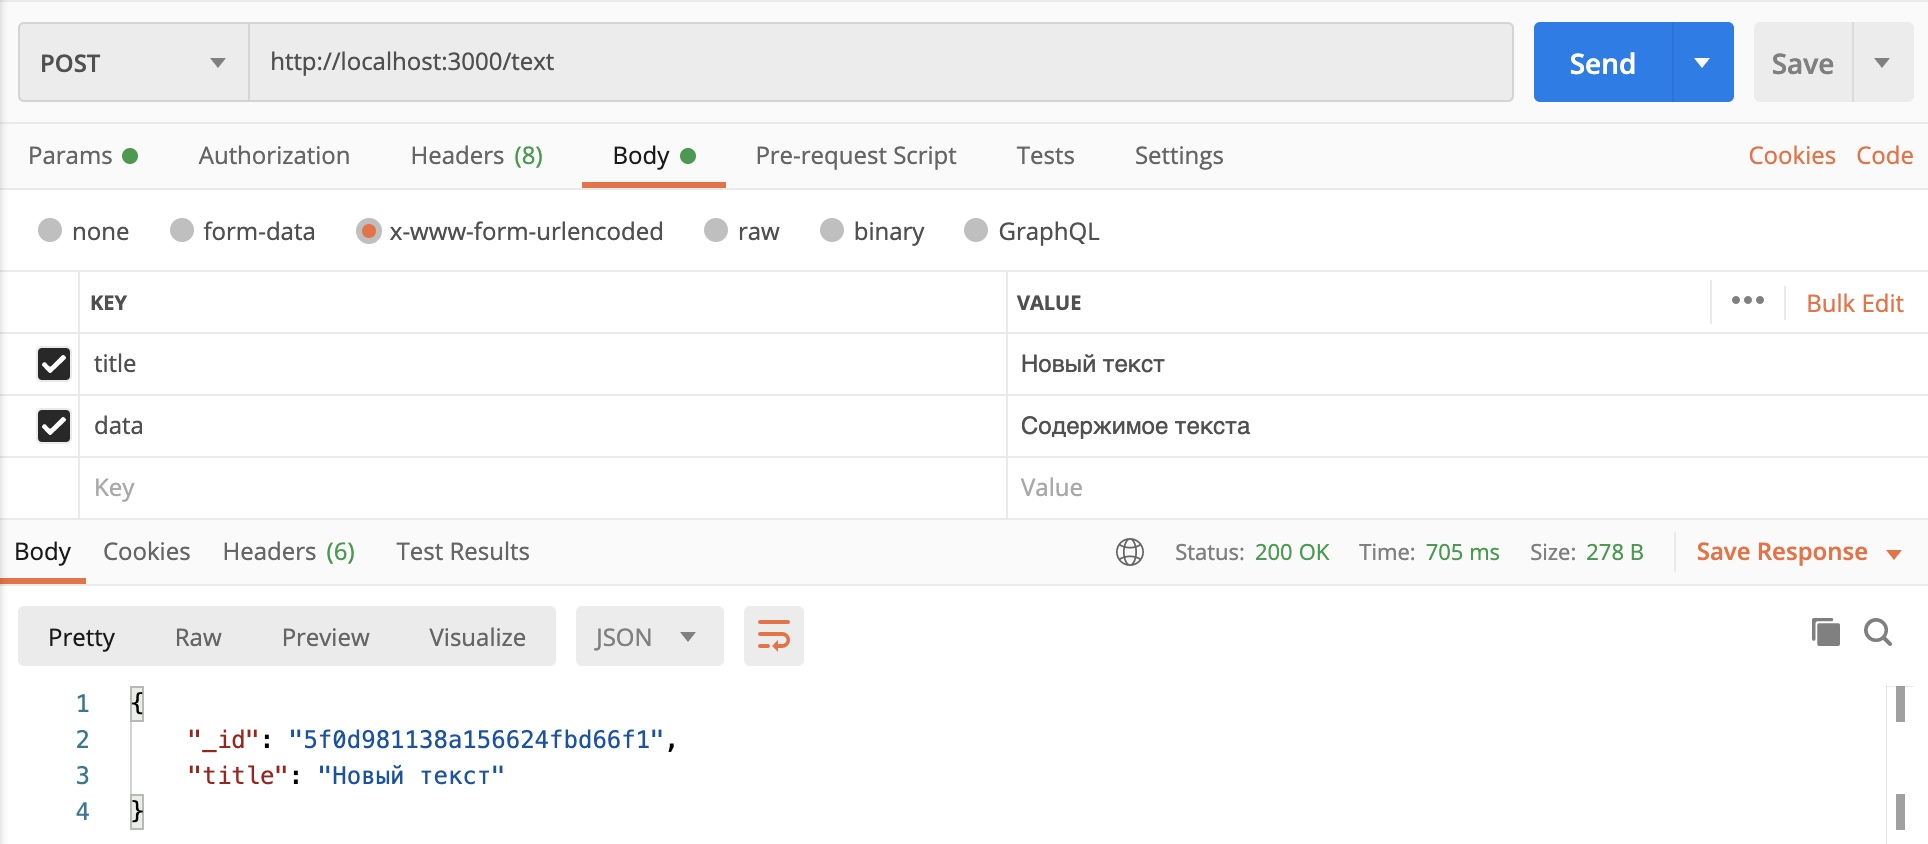
\includegraphics[scale=0.25]{2}

Отправим post запрос с телом title:test и каким то текстом в data. Судя по описанию api приложение должно вернуть мне структуру с id нового обьекта, а также его title. Что и отображается ниже в body, правее указывается код операции - 200, запрос прошел успешно, также вес письма и время выполнения.

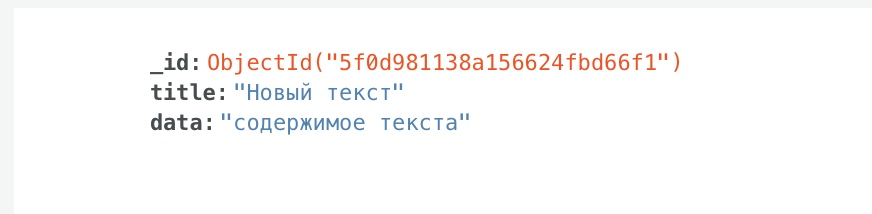
\includegraphics[scale=0.25]{3}

Если мы зайдем на mLab в коллекцию text, мы увидем новый обьект с id, который совпал с вернувшейся id в структуре.

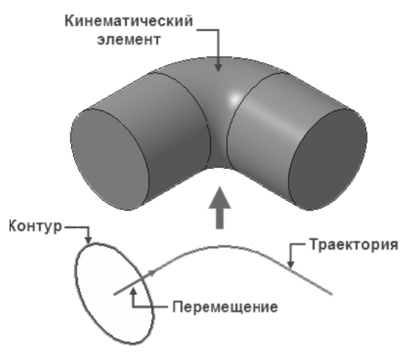
\includegraphics[scale=0.25]{1}

В примере выше мы отправили get запрос на url localhost:3000/search с атрибутами title и pattern, что же делает в этом случае сервер?

\begin{lstlisting}[language=JavaScript]
app.get('/search', (req, res, next) => {
    if (!req.body.title) {
        next();
    } else {
        const details = {title: req.body.title};
        db.collection('text').findOne(details, (err, item) => {
            if (err) {
                res.send({ 'error': 'An error has occured' });
            } else {
                var re = Shingl(req.body.pattern.toLowerCase(), item.data);
                res.send({ result: re });
            }
        });
    }
});
\end{lstlisting}

Приложение регестрирует url /search, так как функция обработки является асинхронной, вызывать код последовательно бесполезно, поэтому используем callback с параметрами req (тело запроса), res(тело ответа) и next(следующий middleware, если текущий не сможет обработать запрос).

Делается запрос к базе данных по нужному фильтру, ответ уходит в callback, на основании ответа формируется ответ, либо ответ процента плагиата, либо код и тело ошибки.

На фотографии Postman мы видим ответ, в разделе body, вернул нам структуру с result равным 0.78.




\section*{Ссылка на GitHub}

https://github.com/pagamov/4sem/tree/master/summer\%20task

\pagebreak